\documentclass[8pt,landscape]{article}

% PACKAGES
\usepackage[letterpaper, margin=0.1in]{geometry}
\usepackage{amsmath, amssymb, geometry}
\usepackage{multicol}
\usepackage{setspace}
\usepackage{sectsty}
\usepackage{verbatim}
\usepackage{graphicx}
\usepackage{xcolor}
\usepackage{listings}
\usepackage{enumitem}
\usepackage{booktabs} % For better tables if needed

% Define a custom color for code highlighting and environment
\definecolor{myred}{RGB}{204, 0, 0} % A strong red
\definecolor{mygray}{RGB}{240, 240, 240} % Light gray for background
\setlist[itemize]{
    noitemsep,  % Removes vertical space between list items
    topsep=0pt,  % Removes space before the list
    partopsep=0pt, % Removes extra space when a list begins mid-paragraph
    parsep=0pt, % Removes space between paragraphs within an item
    leftmargin=*, % Sets the left margin to the minimum necessary
    labelsep=0.5em, % You can slightly adjust the space between the bullet and the text
}
% LISTINGS SETUP for R and Python
\lstset{
  basicstyle=\ttfamily\scriptsize\color{black},
  backgroundcolor=\color{mygray},
  frame=single,
  frameround=tttt,
  framesep=0pt,        % no padding between code and frame
  rulecolor=\color{black!20},
  rulesep=0pt,         % no space between rules
  breaklines=true,
  columns=fullflexible,
  showstringspaces=false,
  commentstyle=\color{gray},
  keywordstyle=\color{blue!80!black},
  stringstyle=\color{myred},
  breakatwhitespace=true,
  xleftmargin=0pt,     % no left margin
  xrightmargin=0pt,    % no right margin
  aboveskip=0pt,       % no space above listing
  belowskip=0pt,       % no space below listing
  abovecaptionskip=0pt,
  belowcaptionskip=0pt,
  framexleftmargin=0pt,
  framexrightmargin=0pt,
  framextopmargin=0pt,
  framexbottommargin=0pt
}

% FORMATTING
\setstretch{0.9} % Reduce line spacing
\setlength{\parindent}{0pt}
\setlength{\parskip}{0pt}

% Reduce section spacing and change color
\makeatletter
\renewcommand{\section}{\@startsection{section}{2}{0pt}%
    {0.1ex}% space before section
    {0.1ex}% space after section
    {\fontsize{8}{9}\bfseries\color{red}}} % section font: 8pt
\makeatother

% Reduce subsection spacing and make subsections blue
\makeatletter
\renewcommand{\subsection}{\@startsection{subsection}{2}{0pt}%
    {0.1ex}% space before subsection
    {0.1ex}% space after subsection
    {\fontsize{8}{9}\bfseries\color{blue}}} % Subsection font: 8pt
\makeatother

% Custom command for red-highlighted code/commands (for in-line use)
\newcommand{\code}[1]{\textcolor{myred}{\texttt{#1}}}

% Custom small text wrapper - ensuring 8pt for body text
\newcommand{\smalltext}[1]{
  {\fontsize{8}{9}\selectfont\sloppy #1\par}
}

% DOCUMENT START
\begin{document}
\fontsize{8}{9}\selectfont % Set the base font size to 8pt and line skip to 9pt for the entire document
\pagestyle{empty}
\begin{multicols}{3}

\section{Causal Inference Objectives}
\smalltext{
Distinguishing between \textbf{experimentally-generated} and \textbf{observational data} to evaluate causal claims. Key goals include fitting regression models that adjust for \textbf{confounding variables} and applying the principle: \code{block what you can, randomize what you cannot} in experimental designs like A/B testing.
}

\textbf{Relevance to Data Science}
\smalltext{
This block emphasizes \textbf{"joined-up thinking"} across the data pipeline. It covers randomized studies, such as \textbf{A/B testing} for website optimization, and non-randomized studies, such as assessing drug efficacy in large healthcare databases.
}

\section{Hypothesis Testing Review}

\smalltext{
\setlength{\tabcolsep}{4pt} % Reduces padding to fit column
\renewcommand{\arraystretch}{1} % Adds vertical breathing room
\begin{tabular}{|p{2.2cm}|c|c|}
\hline
\textbf{Decision} & \textbf{$H_0$ is True} & \textbf{$H_0$ is False} \\ \hline
\textbf{Fail to Reject} & \begin{tabular}[c]{@{}c@{}}Correct (TN)\end{tabular} & \begin{tabular}[c]{@{}c@{}}Type II Error (FN / $\beta$)\end{tabular} \\ \hline
\textbf{Reject $H_0$} & \begin{tabular}[c]{@{}c@{}}Type I Error (FP / $\alpha$)\end{tabular} & \begin{tabular}[c]{@{}c@{}}Correct (TP / Power)\end{tabular} \\ \hline
\end{tabular}
}

\smalltext{
($H_0$) represents the status quo in our case study, whereas ($H_a$) represents our hypothesis of interest.

The \textbf{p-value} is the probability of obtaining a test statistic as extreme as observed, assuming $H_0$ is true. Reject $H_0$ if \code{p-value < alpha}.
The significance level $\alpha$ will be our tolerance to type I error: rejecting the null hypothesis when in fact is true.

\textbf{Increasing Power ($1 - \beta$):} Power is the ability to detect a real effect when it exists (reducing Type II errors). Increasing power helps you find true positives, but it doesn't stop "fake" positives from appearing due to multiple testing.
}

\begin{lstlisting}[language=R]
hypothesis.test <- function(alpha = 0.05, p_value) {
  reject <- (p_value < alpha)
  return(reject)}
\end{lstlisting}

\subsection{P-Hacking \& Type 1 Error Inflation}
\smalltext{
\textbf{p-hacking} is conducting many tests and only reporting significant results ($p < 0.05$). This inflates Type I error. For $m$ independent tests, the probability of at least one Type I error is $1 - (1 - \alpha)^m$.
}

\section{Bonferroni Correction}
\subsection{Family-Wise Error Rate (FWER)}
\smalltext{
Sets a stricter significance level: \code{alpha / m}. It ensures the \textbf{FWER} (chance of $\ge 1$ false rejection) is $\le \alpha$.
}

\begin{lstlisting}[language=R]
sum(pval < (sig_alpha / (nvars * nvars))) # Number of rejected H_0

p.adjust(pval, method = "bonferroni") # Bonferroni Adjustment in R
\end{lstlisting}


\subsection{Trade-offs}
\smalltext{
Bonferroni is \textbf{highly conservative}. It significantly increases the risk of \textbf{Type II errors} (missing real effects).
}


\begin{lstlisting}[language=R]
fdr_p <- p.adjust(raw_p, method = "fdr")# FDR/BH Adjustment in R
\end{lstlisting}
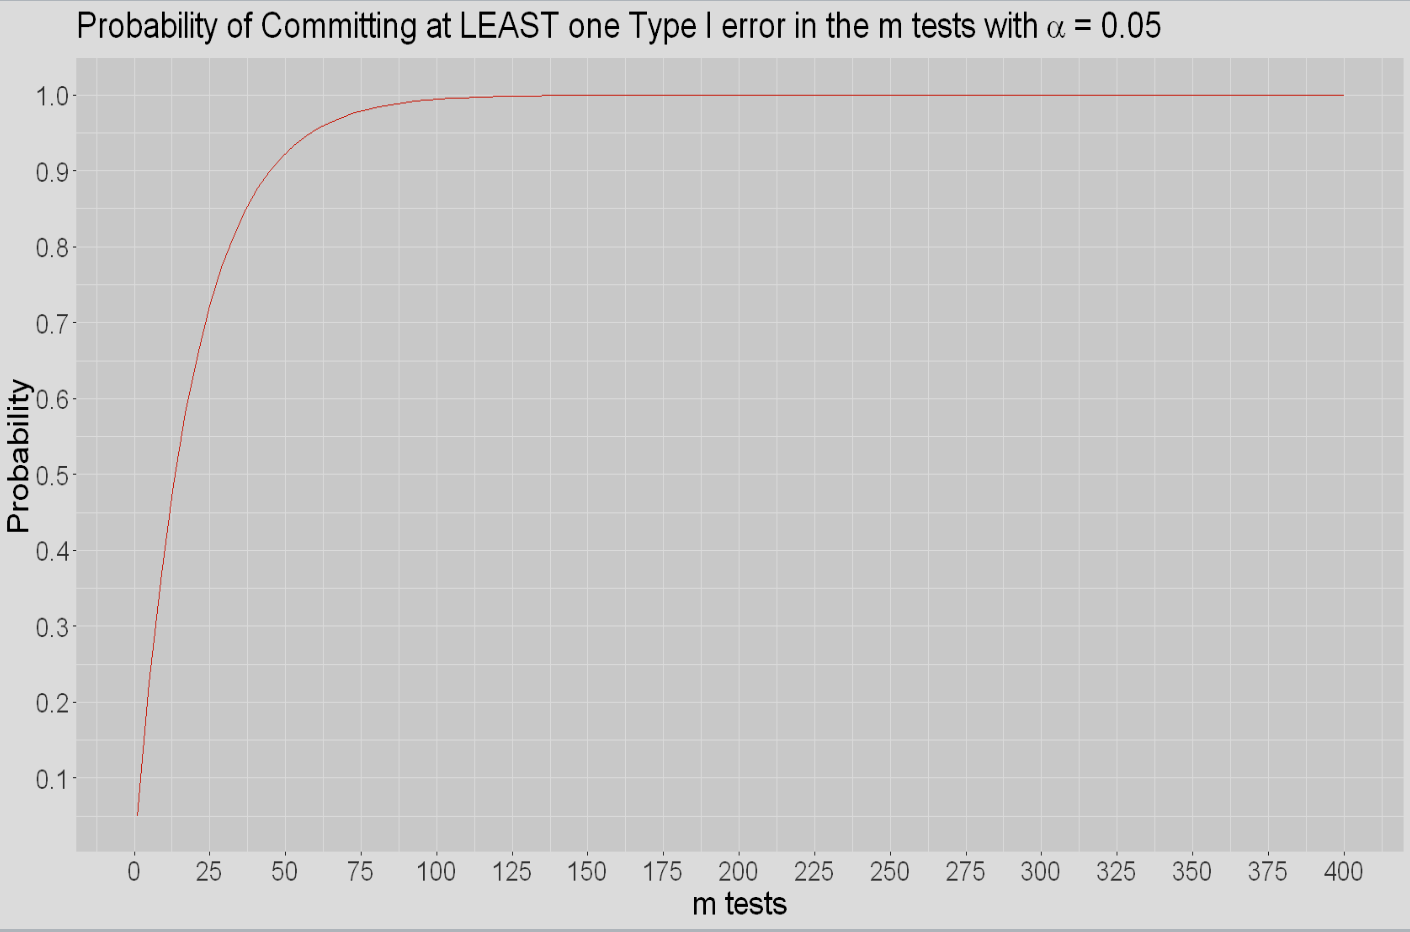
\includegraphics[width=0.50\linewidth, height=2.0cm]{bonf.png}
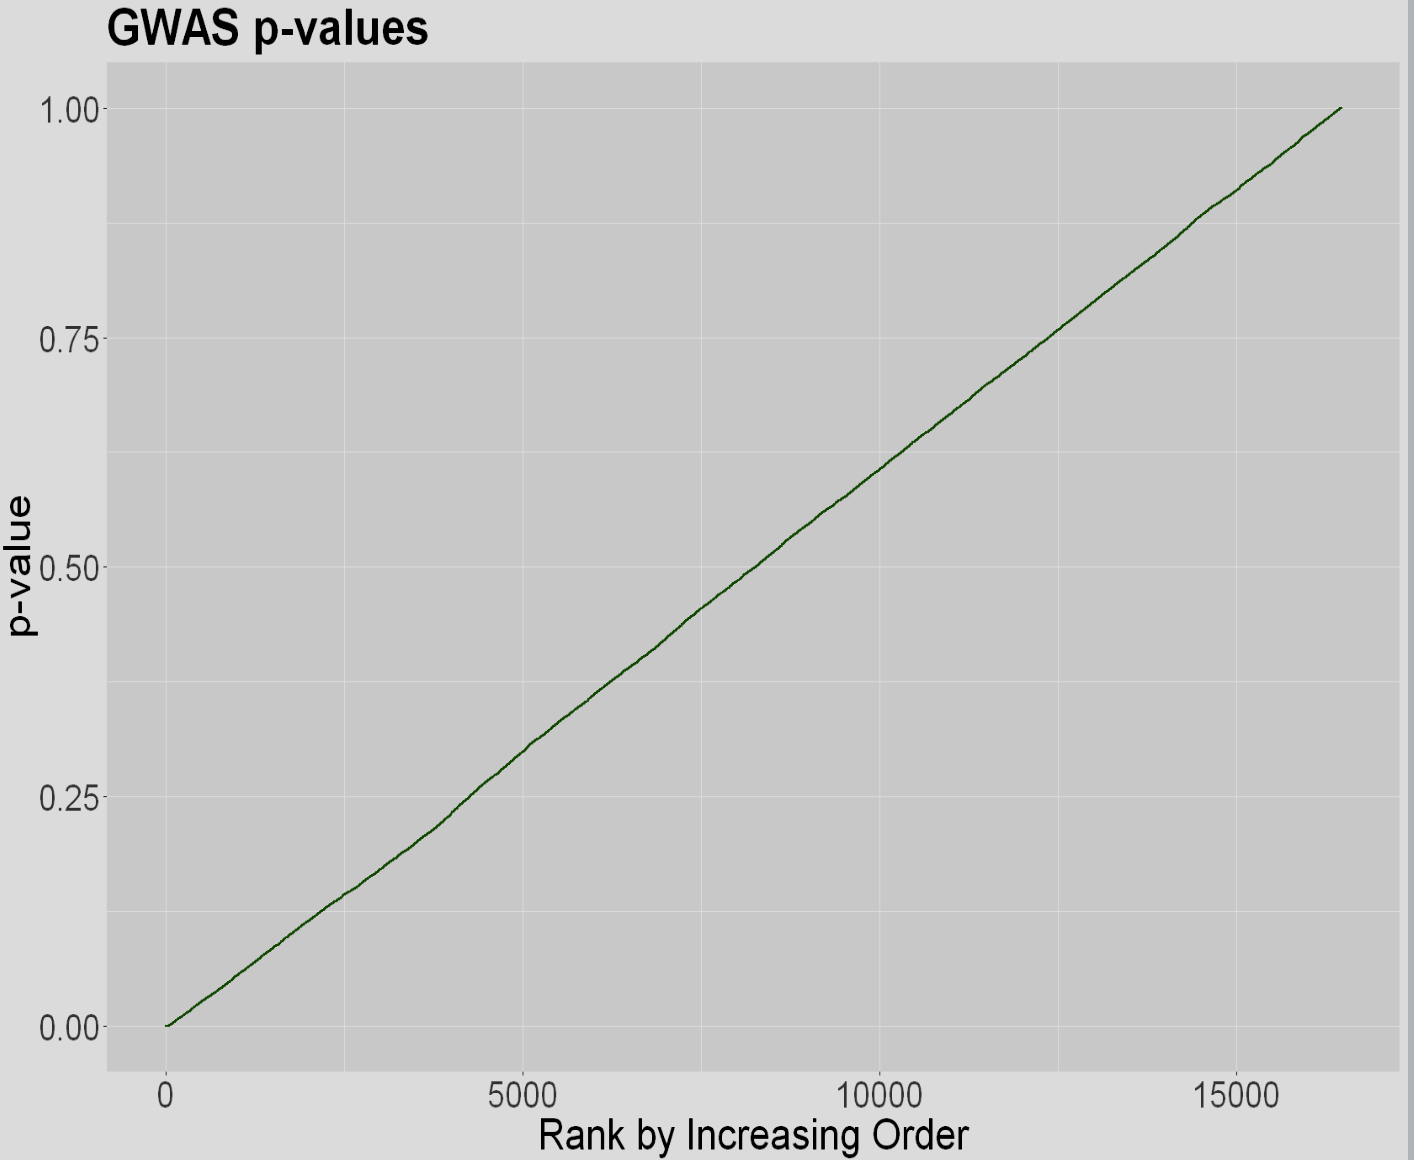
\includegraphics[width=0.50\linewidth, height=2.0cm]{GWAS.png}

\section{False Discovery Rate (FDR)}
\smalltext{
Controls the \textbf{expected proportion of false positives} among all rejections. The \textbf{Benjamini-Hochberg (BH)} method ranks $m$ p-values ($p_{(1)} \le \dots \le p_{(m)}$) and finds the largest $k$ such that $p_{(k)} \le \frac{k}{m}\alpha$.
}

\subsection{Selecting a Correction}
\smalltext{
\textbf{Bonferroni}:if you prefer to be very conservative and would rather miss a real effect than report a fake one.
\textbf{FDR}:if you prefer to be less conservative and want to ensure you don't miss important discoveries, even if it means a small, known percentage of your results might be false positives.
}

\section{Simpson's Paradox}
\subsection{Definition \& Mechanics}
\smalltext{Simpson's paradox occurs when a trend appearing in aggregated data reverses when the data is separated into specific groups. This often results from a limited or poor Exploratory Data Analysis (EDA). A real-world example is COVID-19 fatality rates: Italy appeared to have a higher overall rate than China, but when disaggregated by age, Italy actually had lower rates in every single age group.
}

\section{Confounding Variables}
\subsection{Criteria for Confounding}
\smalltext{
A variable $C$ is a confounder of the relationship between exposure $X$ and outcome $Y$ if:
\begin{itemize}
\item It must be related to the outcome (prognosis or susceptibility).
\item Its distribution must be different in the groups being compared.
\end{itemize}
Confounding is essentially a mixing of effects where the third factor independently affects the risk of the outcome.
}

\begin{lstlisting}[language=R]
# Simulating Simpson's Paradox
simpson_data <- simulate_simpson(n=200, groups=4, r=0.4)

# Overall vs Group correlation
cor(data$X, data$Y) # May be negative
data %>% group_by(Group) %>% 
  summarise(corr = cor(X, Y)) # Positive
\end{lstlisting}

\section{Dealing with Confounding}
\subsection{Observational vs. Experimental}
\smalltext{
\textbf{Observational Studies:} Use stratification or regression adjustment. Include confounders $C$ as additional regressors to "block" their effect. \\
\textbf{Experimental Studies (A/B Testing):} Randomization is the "gold standard." It guarantees that treatment $X$ is independent of all confounders, allowing for causal interpretation.
}

\section{TikTok Simulation Case Study}
\subsection{Naive vs. Precise Modeling}
\smalltext{
The "true" effect of the new ad was an 8-second increase in dwell time.
\begin{itemize}
\item \textbf{Naive Observational}: Effect overestimated (10.68s) because high-dwell-city users chose the new ad.
\item \textbf{Randomized Study}: Comparing "New" vs "Current" yielded an accurate estimate (8.22s).
\item \textbf{ANCOVA}: Including confounders (city/age) in a randomized model increases precision (8.04s with a narrower CI).
\end{itemize}
}

\begin{lstlisting}[language=R]
# Observational with Adjustment
lm(y_obs ~ x_self_choice + city + age, 
   data = sample_TikTok)

# Randomized Study (ANCOVA)
lm(y_exp ~ x_randomized + city + age, 
   data = sample_TikTok)
\end{lstlisting}

\section{Key Takeaways}
\subsection{Causal Inference}
\smalltext{
To avoid misleading conclusions, know how data was collected. Randomization allows accurate estimation without knowing every confounder, but including known covariates (ANCOVA) makes estimations more precise.
}

\end{multicols}
\end{document}